\documentclass[floatsintext,man]{apa6}

\usepackage{amssymb,amsmath}
\usepackage{ifxetex,ifluatex}
\usepackage{fixltx2e} % provides \textsubscript
\ifnum 0\ifxetex 1\fi\ifluatex 1\fi=0 % if pdftex
  \usepackage[T1]{fontenc}
  \usepackage[utf8]{inputenc}
\else % if luatex or xelatex
  \ifxetex
    \usepackage{mathspec}
    \usepackage{xltxtra,xunicode}
  \else
    \usepackage{fontspec}
  \fi
  \defaultfontfeatures{Mapping=tex-text,Scale=MatchLowercase}
  \newcommand{\euro}{€}
\fi
% use upquote if available, for straight quotes in verbatim environments
\IfFileExists{upquote.sty}{\usepackage{upquote}}{}
% use microtype if available
\IfFileExists{microtype.sty}{\usepackage{microtype}}{}

% Table formatting
\usepackage{longtable, booktabs}
\usepackage{lscape}
% \usepackage[counterclockwise]{rotating}   % Landscape page setup for large tables
\usepackage{multirow}		% Table styling
\usepackage{tabularx}		% Control Column width
\usepackage[flushleft]{threeparttable}	% Allows for three part tables with a specified notes section
\usepackage{threeparttablex}            % Lets threeparttable work with longtable

% Create new environments so endfloat can handle them
% \newenvironment{ltable}
%   {\begin{landscape}\begin{center}\begin{threeparttable}}
%   {\end{threeparttable}\end{center}\end{landscape}}

\newenvironment{lltable}
  {\begin{landscape}\begin{center}\begin{ThreePartTable}}
  {\end{ThreePartTable}\end{center}\end{landscape}}




% The following enables adjusting longtable caption width to table width
% Solution found at http://golatex.de/longtable-mit-caption-so-breit-wie-die-tabelle-t15767.html
\makeatletter
\newcommand\LastLTentrywidth{1em}
\newlength\longtablewidth
\setlength{\longtablewidth}{1in}
\newcommand\getlongtablewidth{%
 \begingroup
  \ifcsname LT@\roman{LT@tables}\endcsname
  \global\longtablewidth=0pt
  \renewcommand\LT@entry[2]{\global\advance\longtablewidth by ##2\relax\gdef\LastLTentrywidth{##2}}%
  \@nameuse{LT@\roman{LT@tables}}%
  \fi
\endgroup}


  \usepackage{graphicx}
  \makeatletter
  \def\maxwidth{\ifdim\Gin@nat@width>\linewidth\linewidth\else\Gin@nat@width\fi}
  \def\maxheight{\ifdim\Gin@nat@height>\textheight\textheight\else\Gin@nat@height\fi}
  \makeatother
  % Scale images if necessary, so that they will not overflow the page
  % margins by default, and it is still possible to overwrite the defaults
  % using explicit options in \includegraphics[width, height, ...]{}
  \setkeys{Gin}{width=\maxwidth,height=\maxheight,keepaspectratio}
\ifxetex
  \usepackage[setpagesize=false, % page size defined by xetex
              unicode=false, % unicode breaks when used with xetex
              xetex]{hyperref}
\else
  \usepackage[unicode=true]{hyperref}
\fi
\hypersetup{breaklinks=true,
            pdfauthor={},
            pdftitle={Measuring Lay Theories of Parenting and Child Development},
            colorlinks=true,
            citecolor=blue,
            urlcolor=blue,
            linkcolor=black,
            pdfborder={0 0 0}}
\urlstyle{same}  % don't use monospace font for urls

\setlength{\parindent}{0pt}
%\setlength{\parskip}{0pt plus 0pt minus 0pt}

\setlength{\emergencystretch}{3em}  % prevent overfull lines


% Manuscript styling
\captionsetup{font=singlespacing,justification=justified}
\usepackage{csquotes}
\usepackage{upgreek}



\usepackage{tikz} % Variable definition to generate author note

% fix for \tightlist problem in pandoc 1.14
\providecommand{\tightlist}{%
  \setlength{\itemsep}{0pt}\setlength{\parskip}{0pt}}

% Essential manuscript parts
  \title{Measuring Lay Theories of Parenting and Child Development}

  \shorttitle{Measuring Parenting Theories}


  \author{Emily Hembacher\textsuperscript{1}~\& Michael C. Frank\textsuperscript{1}}

  % \def\affdep{{"", ""}}%
  % \def\affcity{{"", ""}}%

  \affiliation{
    \vspace{0.5cm}
          \textsuperscript{1} Stanford University  }

  \authornote{
    Add complete departmental affiliations for each author here. Each new
    line herein must be indented, like this line. Enter author note here.
    
    Correspondence concerning this article should be addressed to Michael C.
    Frank, 450 Serra Mall, Stanford, CA 94301. E-mail:
    \href{mailto:mcfrank@stanford.edu}{\nolinkurl{mcfrank@stanford.edu}}
  }


  \abstract{Enter abstract here. Each new line herein must be indented, like this
line.}
  \keywords{keywords \\

    \indent Word count: X
  }





\usepackage{amsthm}
\newtheorem{theorem}{Theorem}[section]
\newtheorem{lemma}{Lemma}[section]
\theoremstyle{definition}
\newtheorem{definition}{Definition}[section]
\newtheorem{corollary}{Corollary}[section]
\newtheorem{proposition}{Proposition}[section]
\theoremstyle{definition}
\newtheorem{example}{Example}[section]
\theoremstyle{definition}
\newtheorem{exercise}{Exercise}[section]
\theoremstyle{remark}
\newtheorem*{remark}{Remark}
\newtheorem*{solution}{Solution}
\begin{document}

\maketitle

\setcounter{secnumdepth}{0}



\section{Methods}\label{methods}

\subsection{Participants}\label{participants}

\subsection{Material}\label{material}

\subsection{Procedure}\label{procedure}

\subsection{Data analysis}\label{data-analysis}

\section{Results}\label{results}

\section{Discussion}\label{discussion}

\subsection{Study 1: Demographic
Factors}\label{study-1-demographic-factors}

Approaches to parenting are known to differ across cultures and groups.
For example, \ldots{} To better understand whether the parenting
attitudes captured by our survey reflect group differences, we examined
average scores on the PAQ subscales based on demographic factors. We
administered the PAQ to 680 parents who were members of a local
children's museum and subsequently asked them to provide information
about their gender, level of education, age, ethnicity, and the number
of children they have. Figure X displays the distributions of
demographic factors. To quantify any possible group differences, we
conducted separate linear mixed-effects regressions for each subscale
with the following structure:

\texttt{score\ \textasciitilde{}\ age\ +\ education\ +\ ethnicity\ +\ gender\ +\ number\ of\ children\ +\ (1\ \textbar{}\ subject)\ +\ (1\textbar{}\ item)}

\begin{figure}
\centering
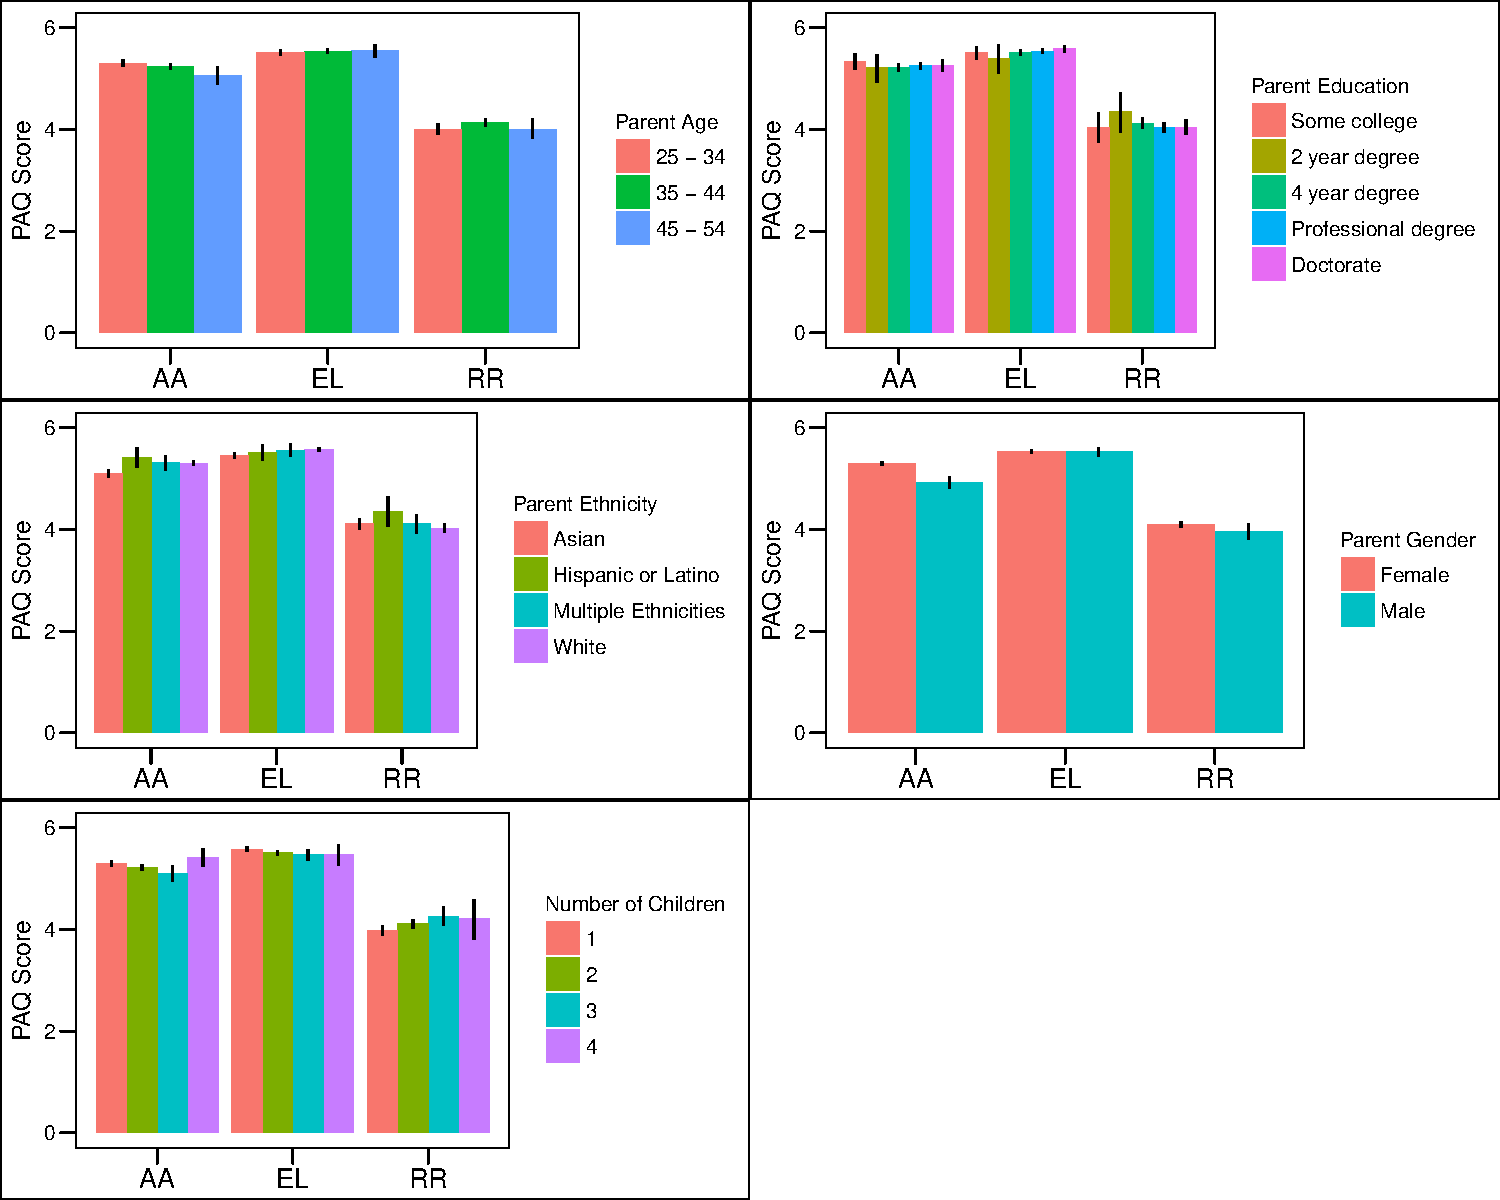
\includegraphics{PAQ_paper_files/figure-latex/unnamed-chunk-11-1.pdf}
\caption{}
\end{figure}

\begin{table}[b]
\centering
\begin{tabular}{llrrrll}
  &  & Estimate & SE & $t$ value & $p$ value &  \\ 
  \hline
Affection and Attachment & Intercept & 5.42 & 0.22 & 25.14 & $<$ .001 & *** \\ 
   & Parent Age & -0.05 & 0.03 & -1.78 & 0.08 & . \\ 
   & Hispanic or Latino & 0.33 & 0.10 & 3.44 & $<$ .001 & *** \\ 
   & Multiple Ethnicities & 0.25 & 0.08 & 3.13 & 0 & ** \\ 
   & White & 0.22 & 0.05 & 4.71 & $<$ .001 & *** \\ 
   & Parent Education & 0.01 & 0.01 & 1.54 & 0.12 &  \\ 
   & Number of children & -0.05 & 0.03 & -2.08 & 0.04 & * \\ 
   & Male & -0.36 & 0.06 & -6.25 & $<$ .001 & *** \\ 
   \hline
Early Learning & Intercept & 5.27 & 0.18 & 29.91 & $<$ .001 & *** \\ 
   & Parent Age & 0.04 & 0.02 & 1.62 & 0.11 &  \\ 
   & Hispanic or Latino & 0.10 & 0.08 & 1.26 & 0.21 &  \\ 
   & Multiple Ethnicities & 0.14 & 0.07 & 2.15 & 0.03 & * \\ 
   & White & 0.14 & 0.04 & 3.73 & $<$ .001 & *** \\ 
   & Parent Education & 0.02 & 0.01 & 2.36 & 0.02 & * \\ 
   & Number of children & -0.06 & 0.02 & -2.66 & 0.01 & ** \\ 
   & Male & -0.03 & 0.05 & -0.66 & 0.51 &  \\ 
   \hline
Rules and Respect & Intercept & 3.85 & 0.34 & 11.33 & $<$ .001 & *** \\ 
   & Parent Age & 0.00 & 0.04 & 0.03 & 0.98 &  \\ 
   & Hispanic or Latino & 0.17 & 0.15 & 1.14 & 0.25 &  \\ 
   & Multiple Ethnicities & -0.03 & 0.13 & -0.20 & 0.84 &  \\ 
   & White & -0.13 & 0.07 & -1.83 & 0.07 & . \\ 
   & Parent Education & -0.01 & 0.01 & -1.11 & 0.27 &  \\ 
   & Number of children & 0.11 & 0.04 & 2.75 & 0.01 & ** \\ 
   & Male & -0.12 & 0.09 & -1.32 & 0.19 &  \\ 
  \end{tabular}
\caption{Results of a linear regression of demographic factors on  PAQ scores.} 
\end{table}

\newpage

\section{References}\label{references}

\begingroup
\setlength{\parindent}{-0.5in} \setlength{\leftskip}{0.5in}

\hypertarget{refs}{}

\endgroup






\end{document}
